\newpage
\section{Gamification Walkthrough}

\subsection{Definition of Levels in Gamification }

\subsubsection{Purpose}
Level is a playable set of questions with content from a single topic that students can play through and earn points. It also allows staff to customise questions, question type, points available and time allowed for each question.

\subsubsection{What was Implemented}
Levels are sets of questions that consist of content from a specific topic within a topic group. Levels can be categorized as Knowledge, Practice and Challenge with increasing difficulty and point earning potential respectively. Levels are built to be reusable and customisable by any staff on the platform.

\subsubsection{How it was Implemented}
Levels store general info like name of level, type of level, week it is visible as well as an array of questions in the backend. We can create a level through our backend api built that takes in all the information and creates a level entity stored in postgres database. In gamification, Level is directly related to a topic on a one to one basis, a level should only have content from a single topic and a topic group will encompass multiple levels which are content from multiple topics.

\subsubsection{Considerations}
\begin{itemize}
    \item Levels should be customisable, editable after creation and performant as the platform could be retrieving many levels at once.
    \item Tradeoff between time allocated for entire level vs time allocated per question
Time limit per question increases difficulty and will generate more competition compared to the time limit for the entire level. I have decided to implement the time allocated per question to increase customizability. As points are awarded based on correct answers, this decision also increases the value of points on the platform.
\end{itemize}

\newpage

\subsection{Definition of Topic Groups in Gamification}

\subsubsection{Purpose}
Topic Groups hold information on topics created within the topic group. Topic Groups are read from the wider metalms to present appropriate content to users in the gamification platform.

\subsubsection{What was Implemented}
In gamification, topic groups are pulled from the metalms and enable the system to identify students assigned to topic groups and levels (topics) created within the topic group. With this relationship between topic groups and levels (which are a set of questions on a topic), admins can easily add or remove topics to topic groups and in doing so change which students have visibility of the levels.

\subsubsection{How it was Implemented}
Staff will first select a topic group from a list retrieved from metalms. The staff must then add start and end dates for the term that the topic group will run in. Once this is done, any levels assigned to this topic group will be assigned to all the students that are enrolled in this topic group. For students, the platform retrieves topic groups assigned to them, this is pulled through the backend api from the enrolment table in DB. Using the topic group id, the platform retrieves all levels associated with the topic groups. The frontend will then filter and only display the levels to users that are visible according to its visibility setting customised by admins.

\subsubsection{Considerations}
\begin{itemize}
    \item Levels should be customisable, editable after creation and performant as the platform could be retrieving many levels at once.
    \item T
\end{itemize}

\newpage

\subsection{Accessing Gamification from metalms}
From the homepage of the metalms, students and admins can get to the gamification feature by clicking Gamification on the sidebar.

\begin{figure}[h!]
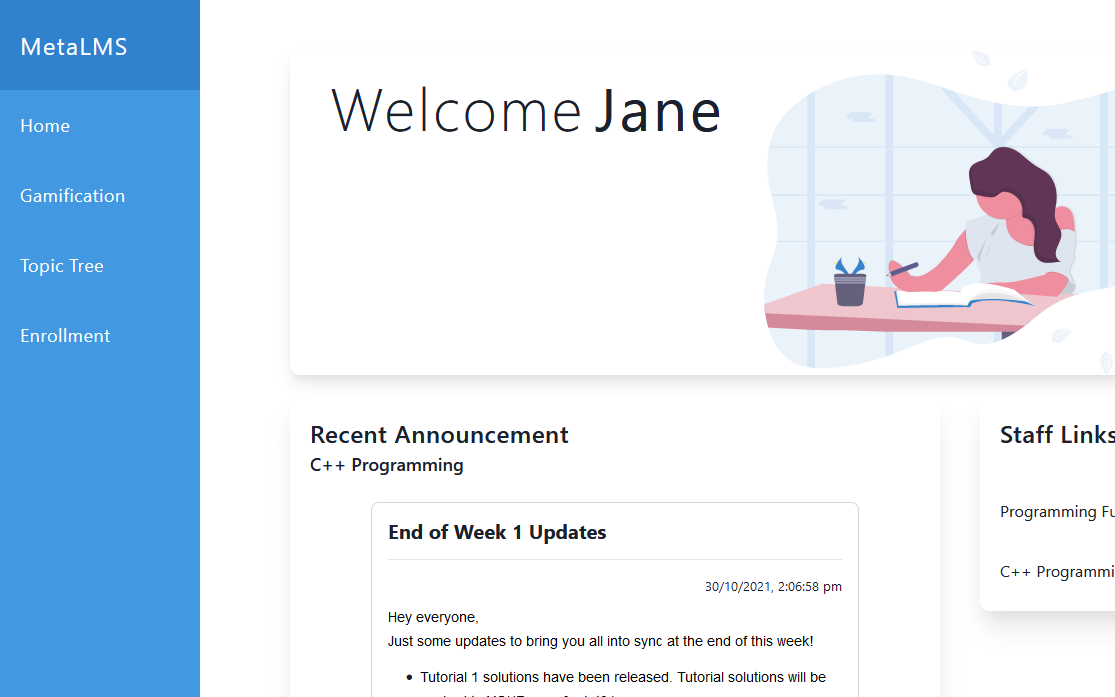
\includegraphics[scale=0.5]{topic-tree-dashboard}
    \centering
    \caption{Accessing Gamification}
\end{figure}


\subsubsection{Purpose}
Serves a connection to the metalms and create a seamless move from metalms to gamification platform

\subsubsection{What was Implemented}
When a user clicks on the gamification link, the system will redirect the user to the gamification feature. Once this redirect occurs, the user's profile metadata is loaded up into the gamification feature as well for a seamless experience.

\newpage

\subsubsection{How it was Implemented}
The metalms has a stored local variable for the authentication token. This token is passed through into the gamification feature which then authenticates the user with the backend database and at the same time retrieves metadata relating to the user. This profile includes user's full name, user's role (Student or Staff), Assigned Topic Groups, Levels Progression and Points Earned. 

\subsubsection{Considerations}
\begin{itemize}
    \item In the final design, I assumed that all users must access the gamification feature through the metalms and cannot seperately login into the gamification system. This was to simplify the routes required and create the integrated experience for users.
    \item A performance and security consideration was how to pass the user from metalms to gamification. Ultimately implemented it based on passing of authentication token which is used to query the backend when user arrived on gamification landing page. This query pulls the user's latest metadata. This has performance impact compared to simply passing the data along, however the security benefit of this outweighed the performance gains that would have been realised.
\end{itemize}

\newpage

\subsection{Student Dashboard}
\subsubsection{Design}
Students will be redirected to the Dashboard page where they can see all the levels assigned to them.

\begin{figure}[h!]
    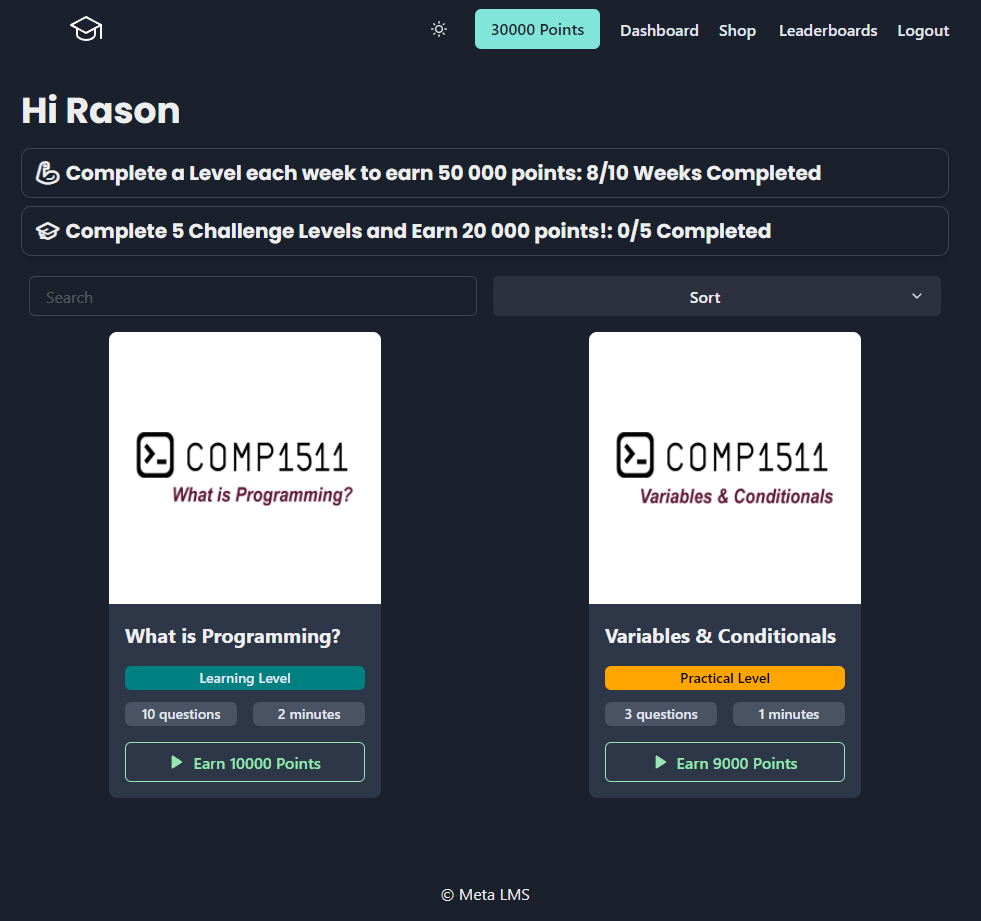
\includegraphics[scale=0.5]{gamification-walkthrough-dashboard}
    \centering
    \caption{Student Dashboard}
\end{figure}

\subsubsection{Purpose}
Provide students an overview of levels available to be played. Provide staff to see the existing levels that they have edit permissions on as well as ability to create new levels.

\subsubsection{What was Implemented}
A grid list of level previews that display the levels available to user. The grid list is searchable to allow users to find specific levels. Level previews display level name, number of questions in level, time allowed and an option to start playing level.

\subsubsection{How it was Implemented}
The system will pull user’s assigned topic groups and populate the levels. Metadata for each level is displayed onto a tile for each level including name of level, duration of level, number of questions and how many points available to be earned. 

\subsubsection{Considerations}
\begin{itemize}
    \item The tile presenting level information should be clear and concise, providing students only information they need.
    \item Decided to implement grid list search and sort functions although it took longer than expected as it allows students to navigate levels easily if there are multiple levels displayed.
    \item Decided to implement view of goals in the dashboard as a combined page as dashboard will ensure students see the goals first before interacting with other functionality.
\end{itemize}

\newpage

\subsection{Starting and Playing a Level}
\subsubsection{Design}
Upon clicking the play button on the level tile on the dashboard page, students will see a get ready page below. Clicking Start Level will move the student to the first question.

\begin{figure}[h!]
    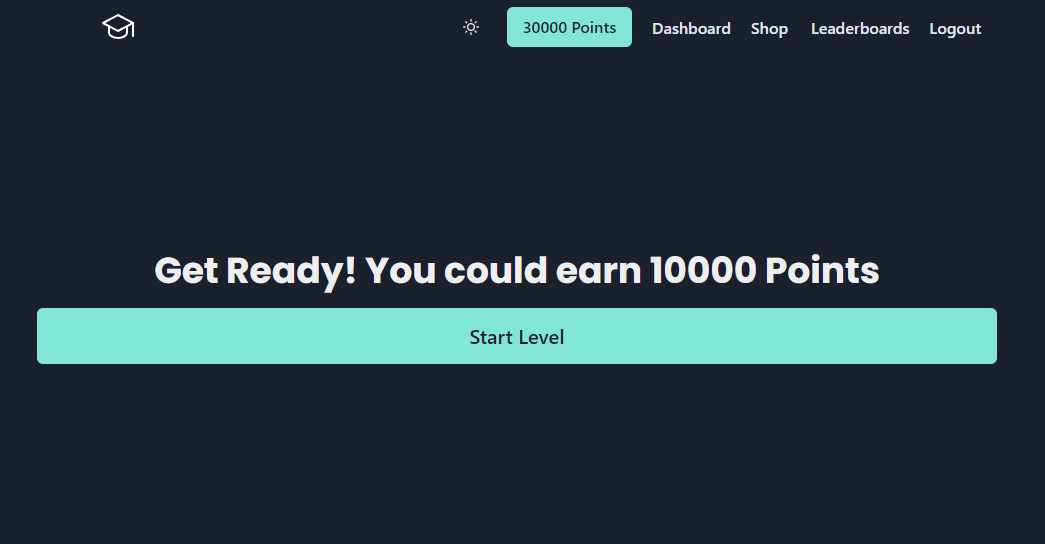
\includegraphics[scale=0.4]{gamification-starting}
    \centering
    \caption{Starting Level}
\end{figure}

Students will be presented with the question and possible answers. They are tasked to select the most correct / appropriate answer. The timer starts the countdown for the time available for this question immediately. Upon reaching 0 time left, the answers will no longer be selectable.

\begin{figure}[h!]
    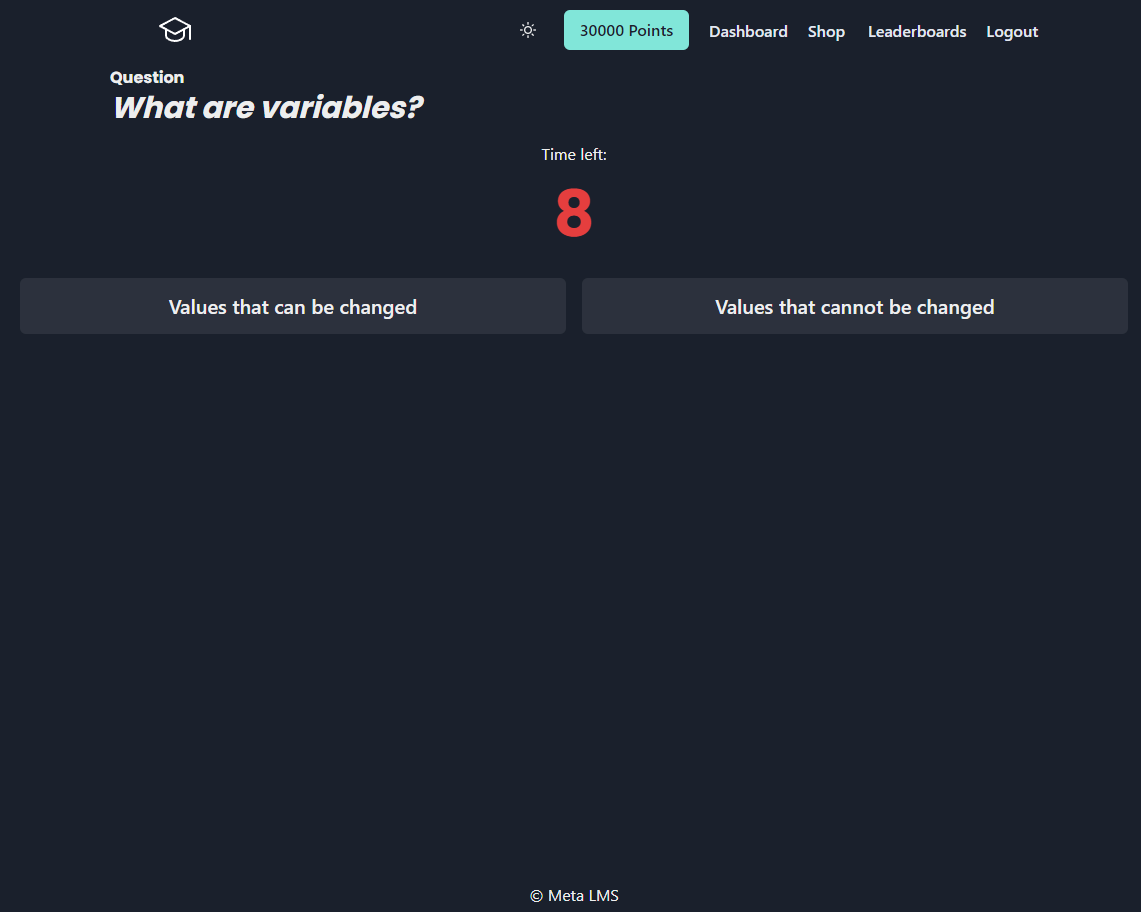
\includegraphics[scale=0.3]{gamification-playlevel}
    \centering
    \caption{Playing Level}
\end{figure}

\newpage

Upon the end of time available for the question, the correct answer is displayed in green and wrong answer displayed in red. The student is also provided with feedback on whether their answer was correct or wrong. If a student did not input an answer, by default their answer is wrong. 
They will be presented with a button to move onto the next question.

\begin{figure}[h!]
    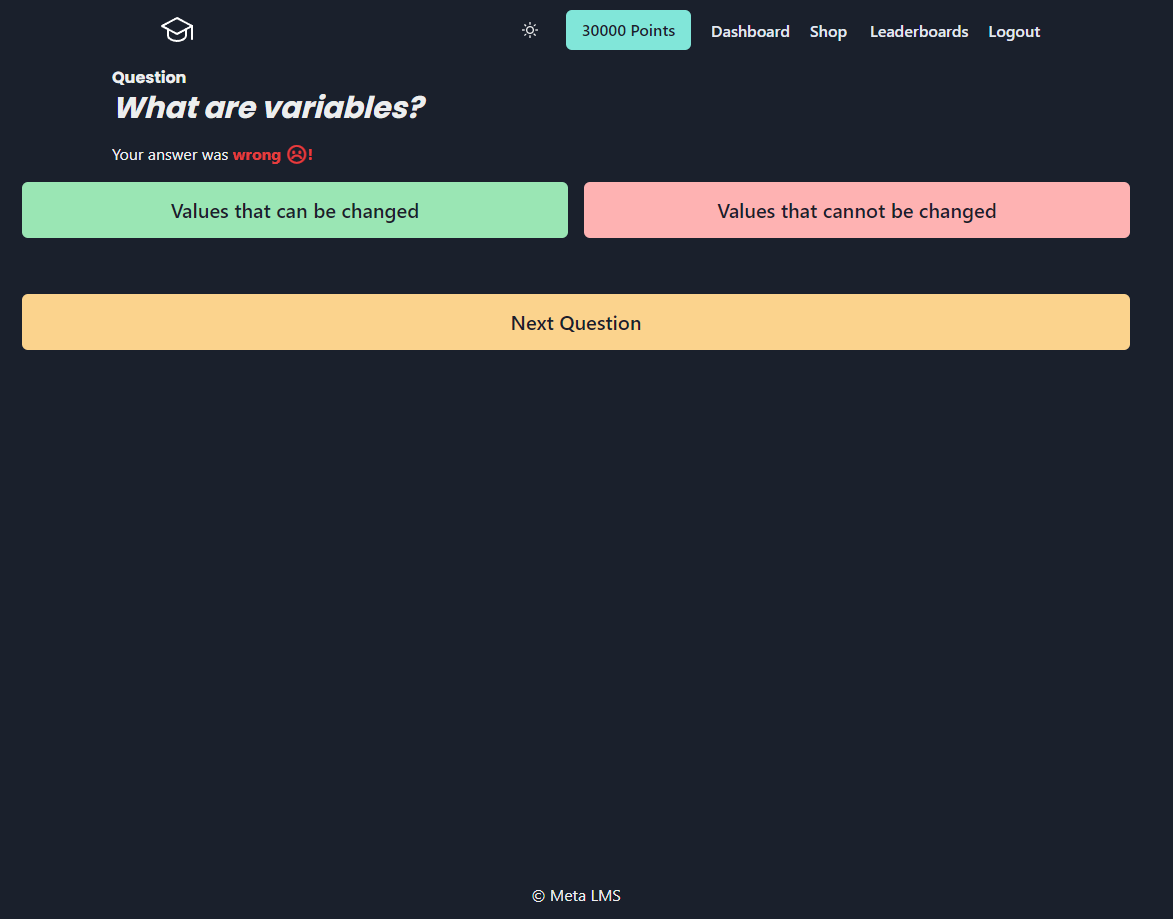
\includegraphics[scale=0.5]{gamification-endquestion}
    \centering
    \caption{End Of Question}
\end{figure}

At the end of the level, students will be presented with an overview of how they performed in the level through correct / wrong outcomes for each question. Additionally, a feedback statement is provided based on the result. If the student has achieved more than 60\% of answers correct, they will see a statement confirming their amount of points earned. If a student achieved between  41\% - 60\% of answers correct, they will see a statement confirming no points awarded. 

\newpage

Finally if a student achieved less than 40\% or lower of answers correct, they will see a statement noting the amount of points penalty applied. The points changes are immediate and students are able to see the new points in the top navigation bar. Additionally, if a student had any boosters active from the shop, their points earned will be adjusted for the effect of the booster. After reading this page, students can return to the dashboard using the return home button.

\begin{figure}[h!]
    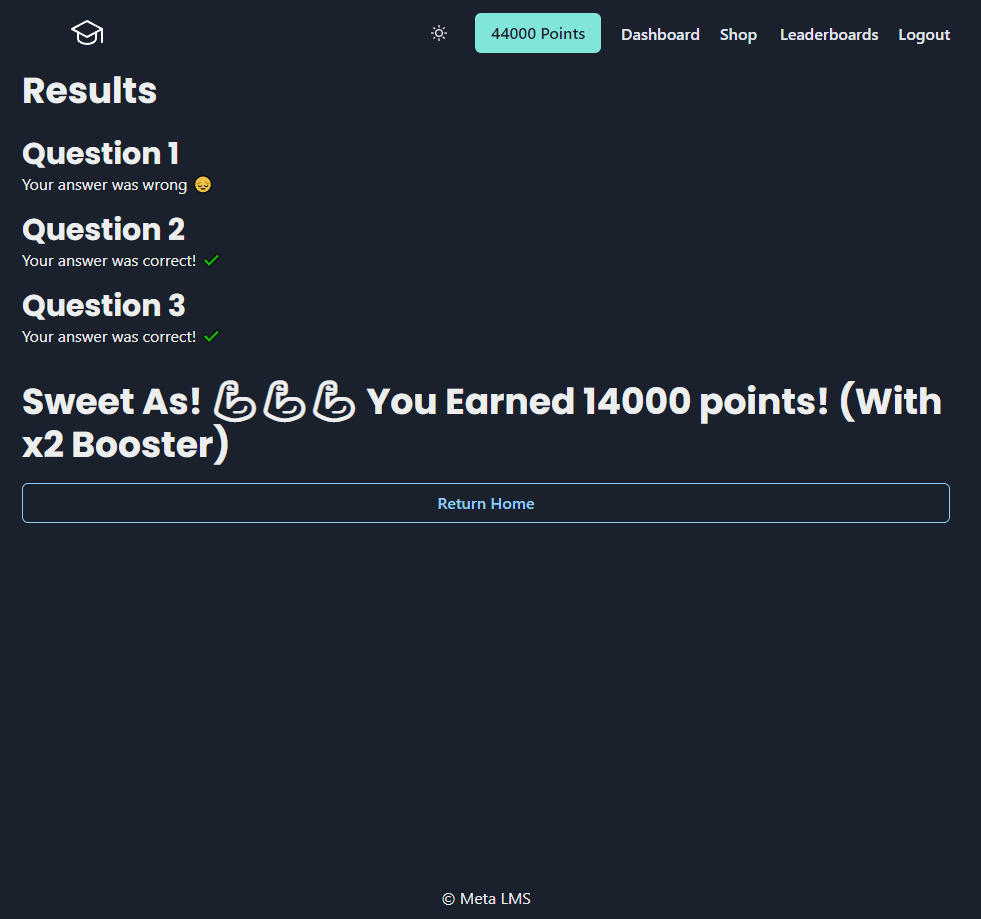
\includegraphics[scale=0.5]{gamification-endlevel}
    \centering
    \caption{End Of Level}
\end{figure}

\newpage

\subsubsection{Purpose}
Playing levels feature enables students to play through the level questions, display time limit per question, review correct answers and determine points earned at end of level.

\subsubsection{What was Implemented}
Students start the playing level feature by clicking play on the selected level. This will bring students to the loading page and subsequently the first question. A countdown timer starts immediately and the question \& answers are displayed. Students can select / change answers until the timer reaches 0 where the UI changes to compare the student's answer to the correct answer and display if the answer was correct. Clicking the next button will allow students to move onto the next question.

After the last question, the feature calculates total points that the user has earned based on the number of questions students have answered correctly / incorrectly. If students answered less than 40\% of questions correctly, they will receive negative points on the questions they answered wrongly. If a student answered between 41\% - 60\% of questions correctly, they do not earn or lose any points. If a student answers more than 60\% of questions correctly, they will earn points based on the questions that they answered correctly.


\subsubsection{How it was Implemented}
Upon clicking the play button on a level, the platform uses the level id to retrieve the questions with respective time allocated, answers for each question and points available for each question. During this process, the user can observe a loading wheel followed by a screen that tells students the maximum amount of points they can earn for the specific level. Students will then be able to click start to begin the level.

Students will then see the first question. The platform will create a countdown timer using the time allocated for the question. During this time before countdown ends, if the user selects an answer, the platform updates selected answers state and sends it off to the backend to ensure that all changes in answers are captured immediately instead of at the end of the countdown. Once the timer ends, it updates the state and locks the selection of answers, it will then compare if selected answers are equal to the answers for the question. If incorrect, it will display “Your answer was wrong”, if correct, it will display “Your answer was correct”. In the background, the platform stores the selected answers back into the backend server and sets a completion timestamp for the question. This same pattern is reused until the last question has been answered. 

\newpage

At the results page, the platform retrieves the latest snapshot of a student's answers and calculates the points earned by the student. This is then validated to find out which category the result falls into (40\%, 41\%-60\%, 61\% - 100\%) and determines a points result which could be negative, 0 or positive. In the background, the platform automatically updates student’s points with the points result. This is how a user loses, earns or maintains their points when playing through a level.

\subsubsection{Considerations}
\begin{itemize}
    \item Student's selected answers are recorded into the system immidiately when they select / change the answer. This deisgn inherently causes more requests to the backend api as students may change answers multiple times during the question compared to keeping the state locally and update backend at the end of the countdown. Ultimately decided with the frequent update due to increased reliability and ensure that changes just before the countdown ends are definitely captured correctly.
    \item The points penalty system took alot of deliberation to design and implement. If there was no penalty to simply guessing the answers for the level, students may not take the levels seriously and make random guesses. However, the system must also be fair to ensure that students who are tryting but struggling are not negatively impacted but rather encouraged to do better. The final design was with the categories of less than or equal to 40\% correct inurring penalty, between 41\% and 60\% answers correct will not earn or lose points and greater than 60\% answers correct will earn points on the answers they got correct.
    \item D
\end{itemize}

\newpage

\subsection{Buying and Using Items from Shop}
\subsubsection{Design}
To access the shop where students can spend their points, they click on the Shop link in the top navigation bar. Once on the shop page, students can see the available items to be purchased using their points. These items are generally to help students earn more points within a set limited time period.

\begin{figure}[h!]
    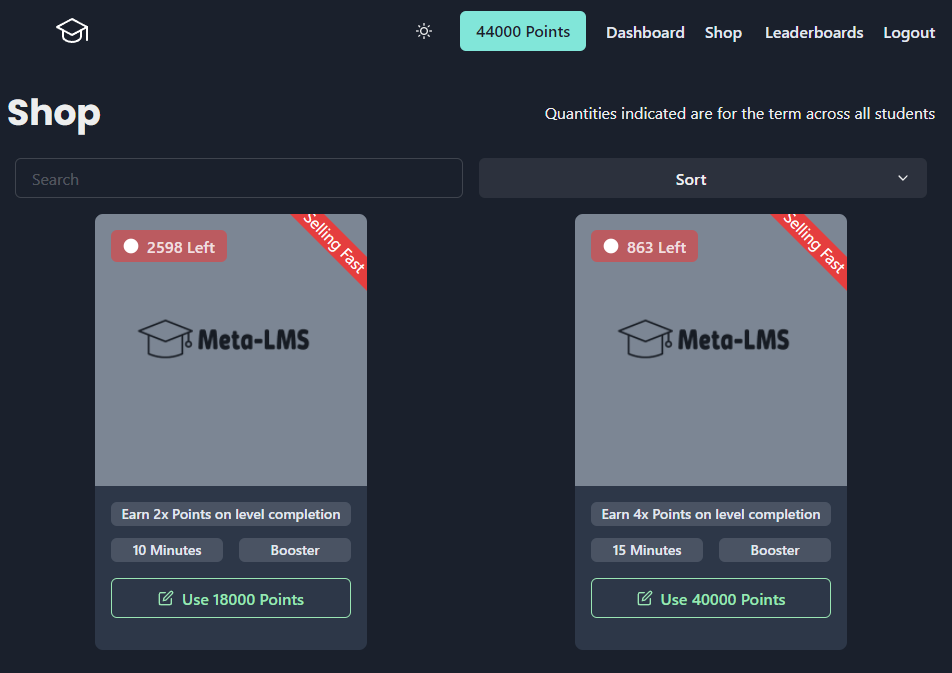
\includegraphics[scale=0.5]{gamification-shop1}
    \centering
    \caption{Browse Shop Page}
\end{figure}

Students can simply select the Use X Points on the specific item they are looking for. The details of the effect and duration of the item is shown on the same tile. Upon clicking Use X Points where X is the number of points it will cost, students will see a confirmation page which will confirm that the booster’s effect will begin immediately. Upon clicking buy, the effect starts and the student will see a banner on the top of the platform to display that the booster is active.

\newpage 

\begin{figure}[h!]
    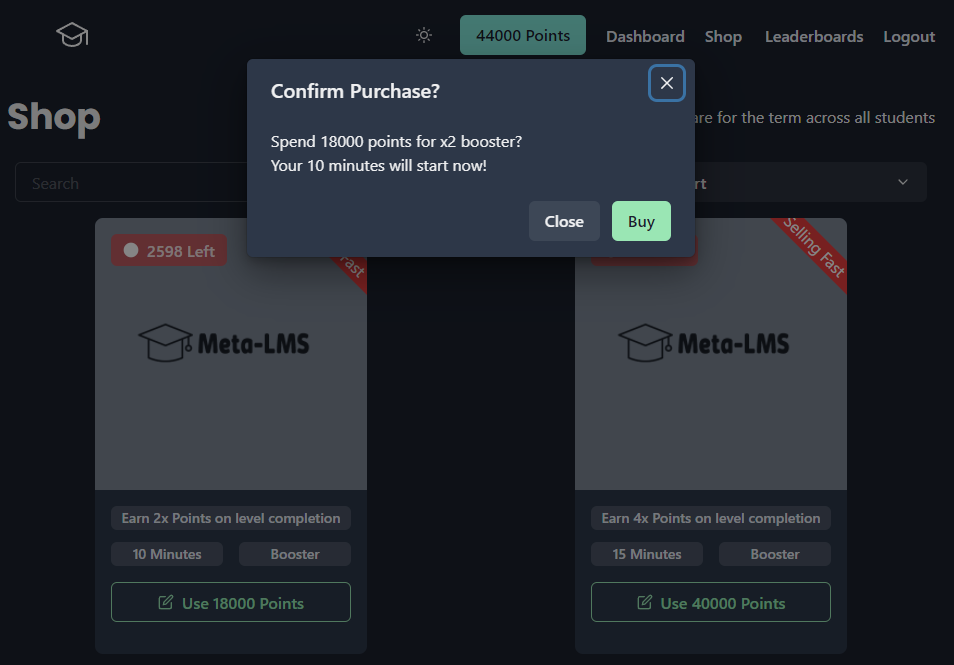
\includegraphics[scale=0.5]{gamification-shop2}
    \centering
    \caption{Buy an Item}
\end{figure}

\begin{figure}[h!]
    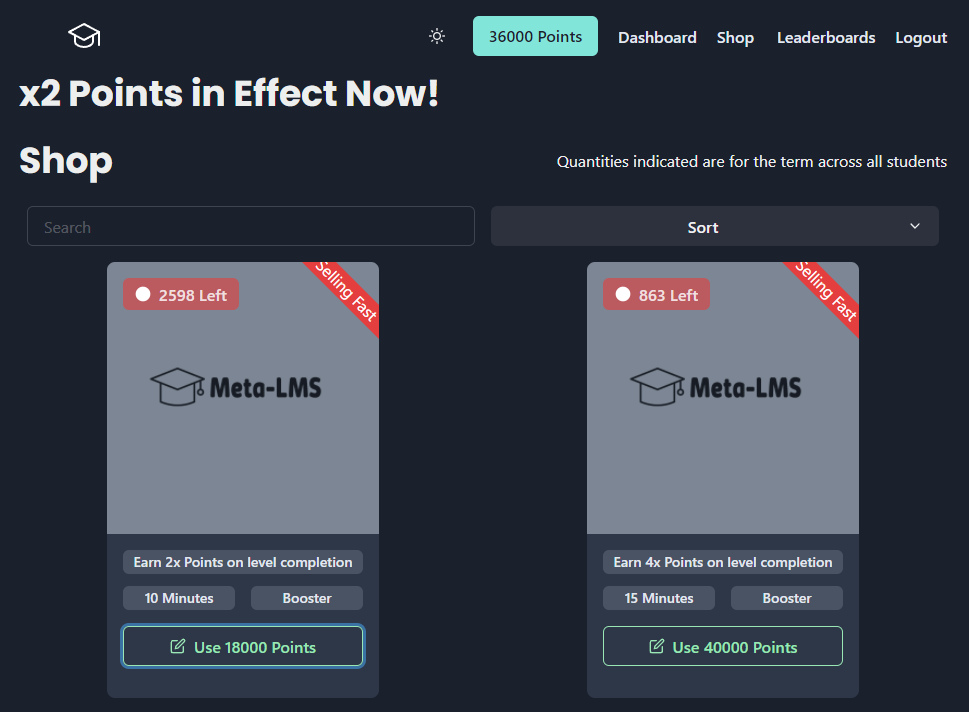
\includegraphics[scale=0.5]{gamification-shop3}
    \centering
    \caption{Shop Item In Effect}
\end{figure}

\newpage

\subsubsection{Purpose}
The shop feature allows students to spend their points on boosters to increase the rate of earning points.

\subsubsection{What was Implemented}
There are 2 boosters available which are x2 points earned and x4 points earned with 10 minutes and 15 minutes duration respectively. These can be easily customised by platform admins and shop items are by default visible to all users on the gamification platform. Users can only buy 1 booster at a time and must use it immediately. Once a booster is used, there will be a banner on the top of the platform to notify users that the booster is in effect, this banner will remain until the effective duration is over. While the booster is in effect, the points that user earned will be multiplied by the multiplier of the booster used.

\subsubsection{How it was Implemented}
Within the backend server, we have a table setup with items. By default only 2 times with the attributes: item name, item type, item duration, item multiplier, item cost. These attributes will change how the booster behaves and the cost required to attain the booster. This information is retrieved when the user navigates to the shop page and the platform will display the items which are available for purchase in a grid list format with an option to buy. In the current implementation, the usage built is only on the item type = booster, it is possible to add other game item types to increase the variety of rewards for points.

\subsubsection{Considerations}
\begin{itemize}
    \item Value of boosters vs the value of points needs to be balanced to drive correct behaviours and competitive environment
\end{itemize}

\newpage

\subsection{Leaderboards}
\subsubsection{Design}
Students can access the leaderboards through the Leaderboards link in the navigation bar. The leaderboards page will display the user’s progress through each of the topic groups that they are part of. It will display a mixture of prescriptive advice for the student to progress further in the platform and provide high level rankings details for the top 3 students in the topic group run to foster a competitive goal for students.

\begin{figure}[h!]
    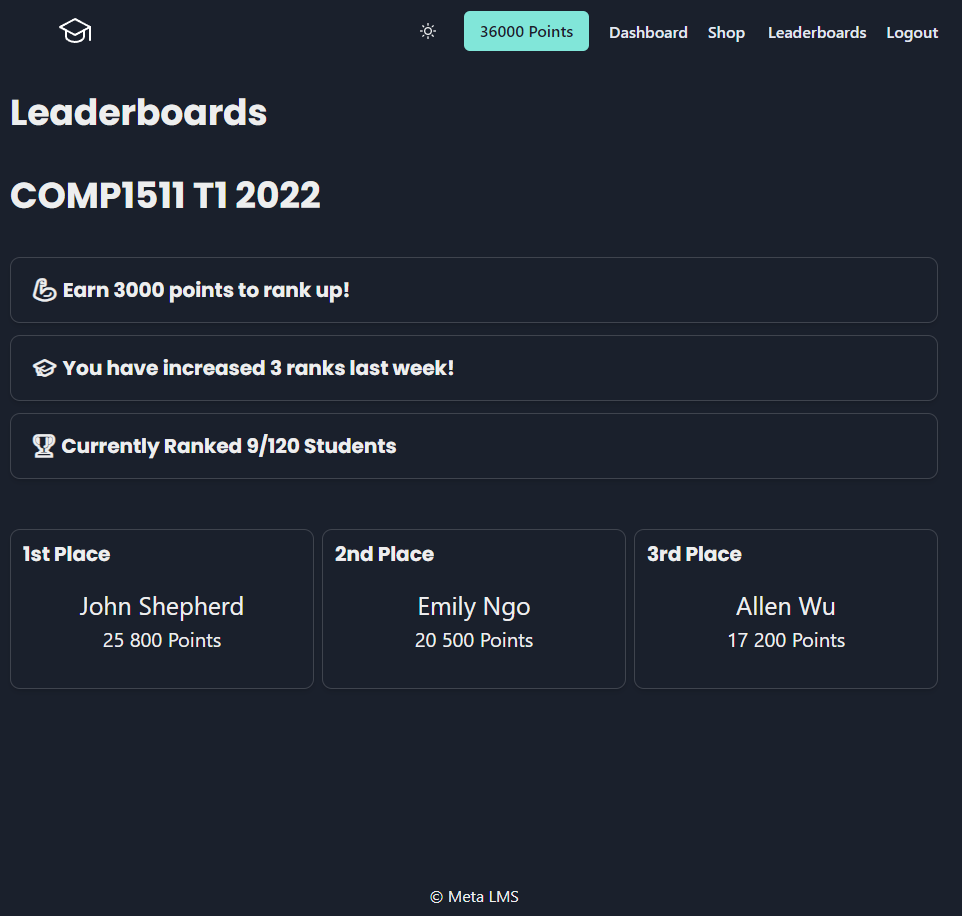
\includegraphics[scale=0.5]{gamification-leaderboards}
    \centering
    \caption{Student Leaderboards}
\end{figure}

\newpage

\subsubsection{Purpose}
Provide students with prescriptive advice to enhance their learning while providing statistics on how they are progressing compared to their peers. This feature aims to create a competitive environment but avoid most of the negative connotations of ranking.

\subsubsection{What was Implemented}
A centralised organisation of statistics that displays to the student their rank in the topic group, how far they are to rank up and also the top 3 students in the topic group. This feature shows these details per topic group so it is more specific and targeted.

\subsubsection{How it was Implemented}
The platform first ranks the user in their topic group based on the amount of points earned on the platform. It then finds out the difference in points to the user in the next higher rank and displays the difference to the student. The system also pulls the details like name, points and ranking of the top 3 students. This is done for each of the topic groups that the student is enrolled in and is displayed one after another in a list format.

\subsubsection{Considerations}
\begin{itemize}
    \item Avoid negative connotations by using a more objective approach to display facts that foster competition
    \item Provide prescriptive advice for students to improve their progress in the platform to break the goal of improvement into small achievable steps.
\end{itemize}

\newpage

\subsection{Creating and Editing Content in Levels}
\subsubsection{Design}
This feature is only accessible by users with role of Staff. Upon entering the gamification platform, users with the assigned role of Admins will be directed to a Levels Dashboard which will display a grid list of all the levels they own / created. There is a button to add a New Level.

\begin{figure}[h!]
    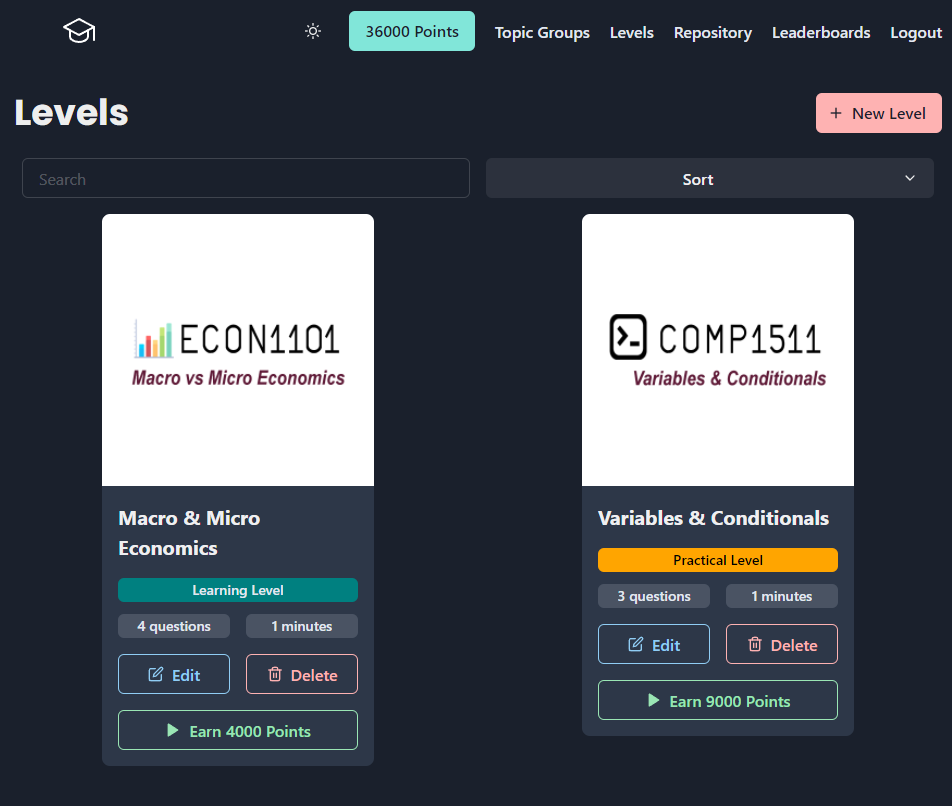
\includegraphics[scale=0.5]{gamification-admin1}
    \centering
    \caption{Admin Levels Dashboard}
\end{figure}

Upon clicking on the New Level button, admins are asked to provide a name for the level in a prompt. Once admin has entered a name for the level, they will be directed to Edit Level Page.

\begin{figure}[h!]
    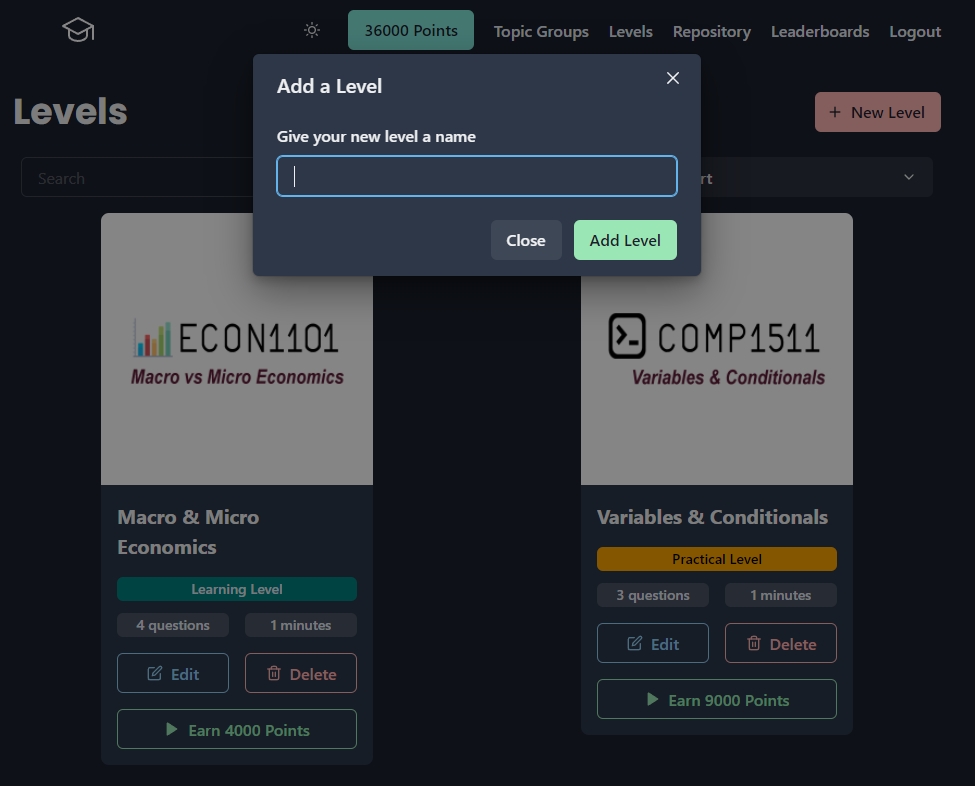
\includegraphics[scale=0.5]{gamification-admin2}
    \centering
    \caption{Create new Level}
\end{figure}

\newpage

Admins are then directed to edit information about the level and its content. This page can be accessed on a new or existing level. Here the admin will add information like level name, week number (determines when in the term the level is visible to students), level type (Knowledge, Practice or Challenge), level format (Level or Live Kahoot Style Quiz) and a Thumbnail for the main image of the level. Below this is a functionality to edit questions that users will see within the level. Clicking Add a question, the user will see questions added with default 10s time available and 1000 points available. These questions can also be easily reordered by dragging the hamburger icon on the left of the tile to move the questions in order with the first question being at the top and last at the bottom.

\begin{figure}[h!]
    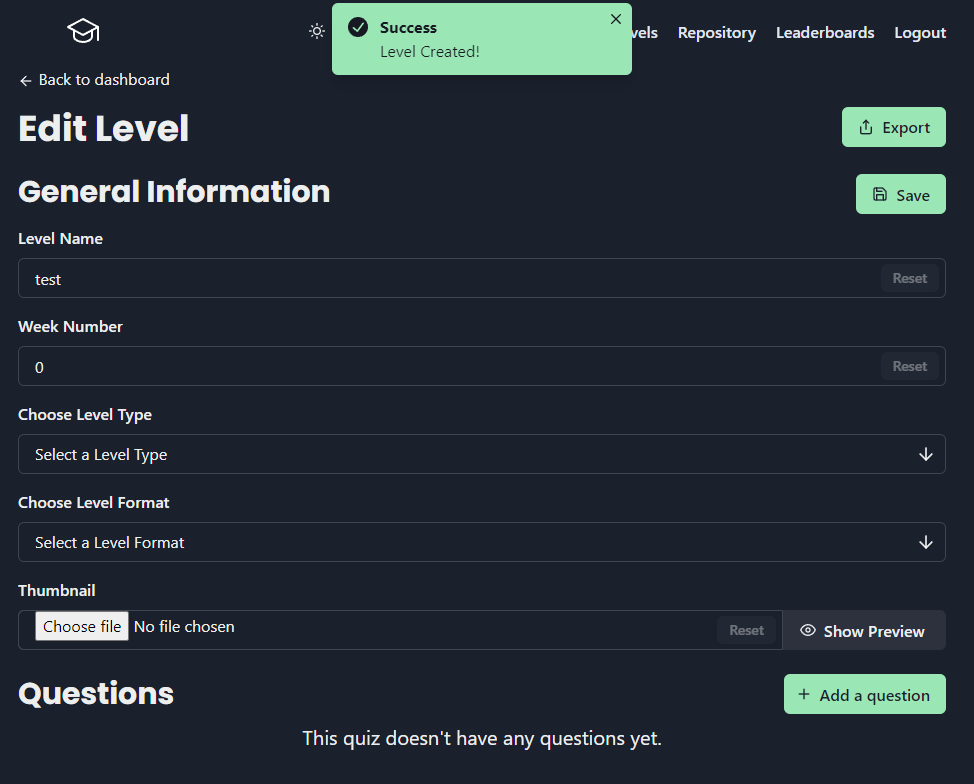
\includegraphics[scale=0.5]{gamification-admin3}
    \centering
    \caption{Create new Level}
\end{figure}

\begin{figure}[h!]
    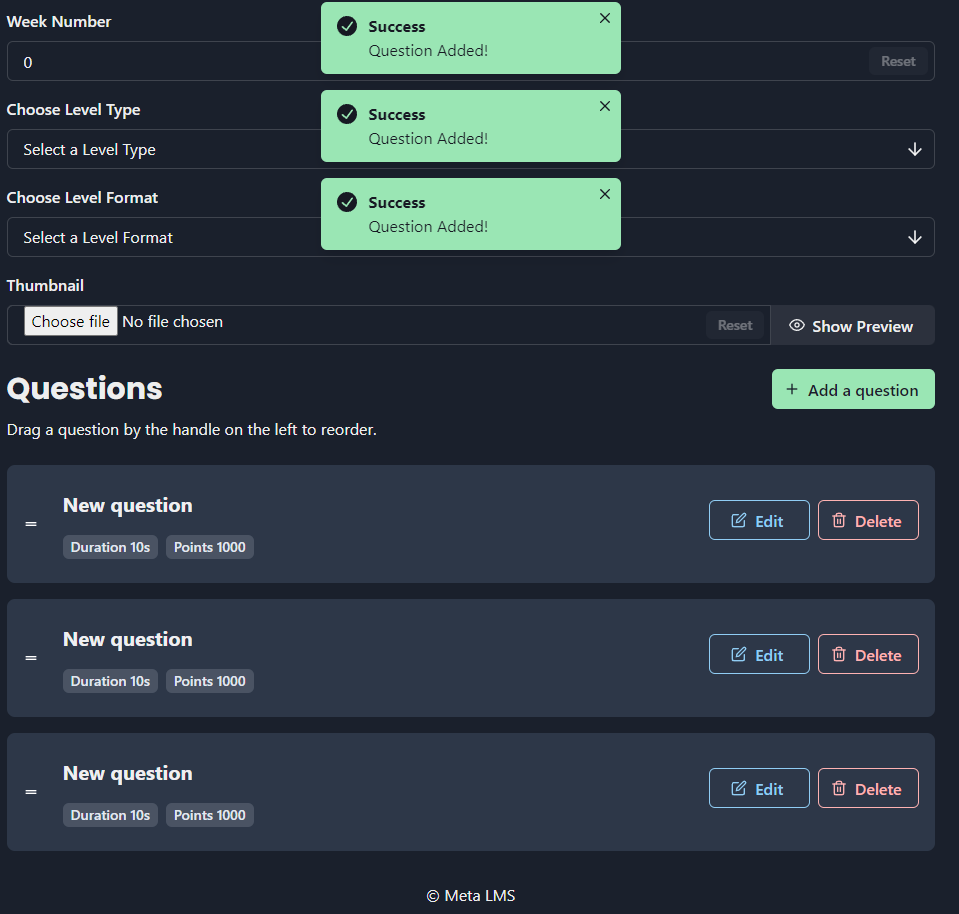
\includegraphics[scale=0.5]{gamification-admin4}
    \centering
    \caption{Create new Level}
\end{figure}

\newpage

Upon clicking edit question, the user will see the edit question page. This page is specific to a single question and allows admin to customise the text for the question, the points available to be earned, the time available (duration) for the question, add any helper media like images or videos and determine the possible answers as well as selecting the correct answers with the green check boxes (can be multiple).

\begin{figure}[h!]
    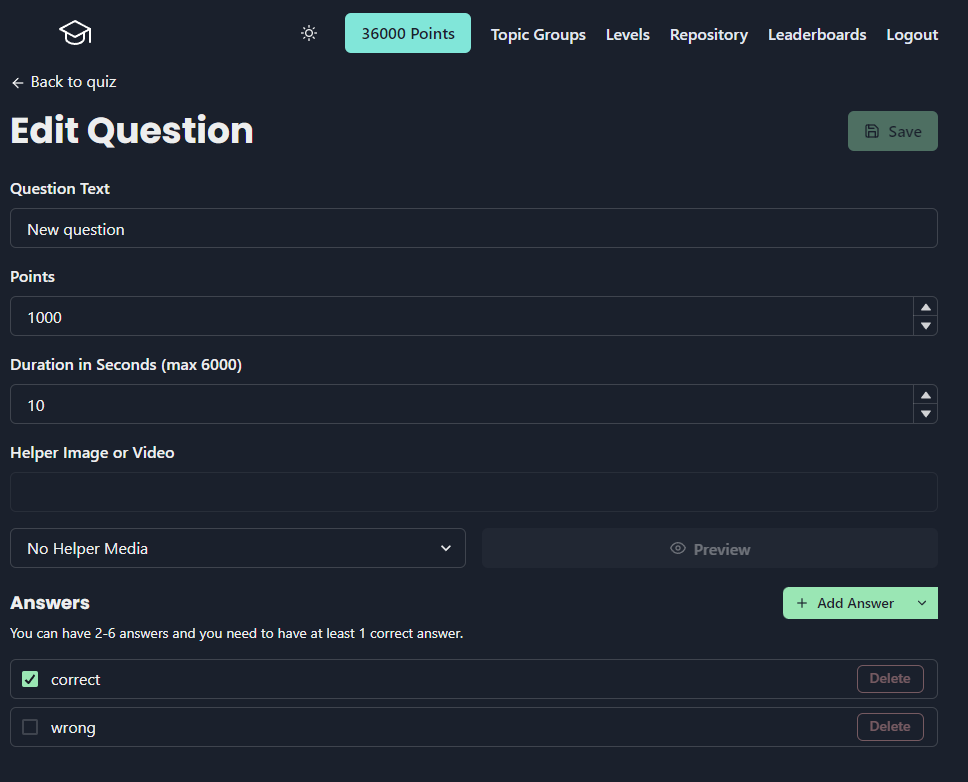
\includegraphics[scale=0.5]{gamification-admin5}
    \centering
    \caption{Create new Level}
\end{figure}


\newpage

\subsubsection{Purpose}
Provide students with prescriptive advice to enhance their learning while providing statistics on how they are progressing compared to their peers. This feature aims to create a competitive environment but avoid most of the negative connotations of ranking.

\subsubsection{What was Implemented}
A centralised organisation of statistics that displays to the student their rank in the topic group, how far they are to rank up and also the top 3 students in the topic group. This feature shows these details per topic group so it is more specific and targeted.

\subsubsection{How it was Implemented}
The platform first ranks the user in their topic group based on the amount of points earned on the platform. It then finds out the difference in points to the user in the next higher rank and displays the difference to the student. The system also pulls the details like name, points and ranking of the top 3 students. This is done for each of the topic groups that the student is enrolled in and is displayed one after another in a list format.

\subsubsection{Considerations}
\begin{itemize}
    \item Avoid negative connotations by using a more objective approach to display facts that foster competition
    \item Provide prescriptive advice for students to improve their progress in the platform to break the goal of improvement into small achievable steps.
\end{itemize}








\newpage